\documentclass[
	% -- opções da classe memoir --
	12pt,				% tamanho da fonte
	openright,			% capítulos começam em pág ímpar (insere página vazia caso preciso)
	oneside,			% para impressão em recto e verso. Oposto a oneside
	a4paper,			% tamanho do papel. 
	% -- opções da classe abntex2 --
	%chapter=TITLE,		% títulos de capítulos convertidos em letras maiúsculas
	%section=TITLE,		% títulos de seções convertidos em letras maiúsculas
	%subsection=TITLE,	% títulos de subseções convertidos em letras maiúsculas
	%subsubsection=TITLE,% títulos de subsubseções convertidos em letras maiúsculas
	% -- opções do pacote babel --
	english,			% idioma adicional para hifenização
	brazil,				% o último idioma é o principal do documento
	]{abntex2}

\usepackage[T1]{fontenc}		% Selecao de codigos de fonte.
\usepackage[utf8]{inputenc}		% Codificacao do documento (conversão automática dos acentos)
\usepackage{indentfirst}		% Indenta o primeiro parágrafo de cada seção.
\usepackage{color}				% Controle das cores
\usepackage{graphicx}			% Inclusão de gráficos
\usepackage{microtype}
\usepackage[alf]{abntex2cite}
\usepackage{mathtools}
\usepackage{amsmath}
\usepackage{listings}
\usepackage{minted}
\usepackage{xcolor}



\tipotrabalho{Relatório técnico}
\renewcommand{\imprimircapa}{%
    \begin{capa}%
        \begin{figure}
            \center
            
\includegraphics[width=2.5cm]{imagens/logo_ufsc.png}
        \end{figure}
        \center
        \ABNTEXchapterfont\large{UNIVERSIDADE FEDERAL DE SANTA CATARINA\\ DEPARTAMENTO DE INFORMÁTICA E ESTATÍSTICA \\ COMPUTAÇÃO GRÁFICA}
        \vfill
        \begin{center}
        \ABNTEXchapterfont\bfseries\LARGE\imprimirtitulo
        \end{center}
        \vfill
        {\ABNTEXchapterfont\large\imprimirautor}
        \vfill
        \large\imprimirlocal
        \large\imprimirdata
        \vspace*{1cm}
        \end{capa}
}

% Informações de dados para CAPA
\titulo{Modelagem Realista de um Objeto de Engenharia: \\ Navio Karl Hoepcke}
% ---------------------------------------------------
%Inserir nomes dos autores aqui
\autor{	Francisco Vicenzi \\
        Gustavo Kundlatsch \\
        \textbf{PROFESSOR} \\ 
        Aldo v. Wangenheim}

% ---------------------------------------------------
\local{Florianópolis \\}
\data{Maio de 2021}
\tipotrabalho{Relatório final}


\definecolor{monokaibg}{HTML}{272822}


\begin{document}
\imprimircapa

\ABNTEXsectionfont
\tableofcontents
\chapter{Conteúdo da Entrega}
    Este relatório possui o detalhamento da experiência do grupo com o uso da ferramenta Blender, bem como a lista de recursos prontos utilizados (tanto objetos quanto texturas). O vídeo da visita virtual foi enviado ao Youtube e os arquivos da modelagem compactados e enviados ao Google Drive. Eles estão disponíveis no link abaixo:

\begin{itemize}
    \item Visita Virtual: \\
    \url{https://www.youtube.com/watch?v=Ej9xQeDoZIA}
    \item Modelagem: \\
    \url{https://drive.google.com/file/d/1NBMiz\_dIEJDnp-tRzbP30ywSWaVH1zxk}
\end{itemize}
\chapter{Experiência do Grupo}
\textual
    Em contrapartida ao trabalho 2, este trabalho mostrou-se um tanto quanto menos desafiador. Um dos principais motivos é que, mesmo com pouco tempo de diferença entre os dois enunciados, já tinha sido possível aprender um pouco sobre o Blender. Além disso, por mais que o jogo desenvolvido tenha sido simples, o Godot Engine mostrou-se bem documentado, com diversos tutoriais e várias coisas intuitivas. 


\chapter{Componentes prontos utilizados}
\textual
    Foi utilizado o modelo do Pokémon Machoke, disponibilizado na página da disciplina e desenvolvido pela ROEstudios. Em relação ao MoCap, foram utilizados os arquivos de 2019-1, em que os movimentos de uma colega, Ana, foram capturados. Por fim, utilizou-se também um modelo de vacina/seringa obtido no seguinte endereço: \url{https://www.blendswap.com/blend/7676}.

As texturas utilizadas no chão e nos muros do mapa foram obtidas em, respectivamente, \url{https://cc0textures.com/view?id=Tiles093} e \url{https://cc0textures.com/view?id=Bricks059}.

\chapter{Resultado final}
\textual
    Fora o navio (e os componentes que fazem parte dele, como mastro, escadas, etc), também foram produzidos dois objetos a parte: um timão e um telégrafo.

O timão e o telégrafo são apresentados na figura \ref{fig:tim_te}. O primeiro andar conta com duas salas. A figura \ref{fig:sala1} apresenta a primeira sala, enquanto a figura \ref{fig:sala2} apresenta a segunda. Na figura \ref{fig:niquel}, temos a sala do segundo andar renderizada. Nessas imagens, são apresentados alguns componentes que obtivemos prontos, como a mesa de sinuca, sofá e caça-níquel.

\begin{figure}[!h]
    \centering
    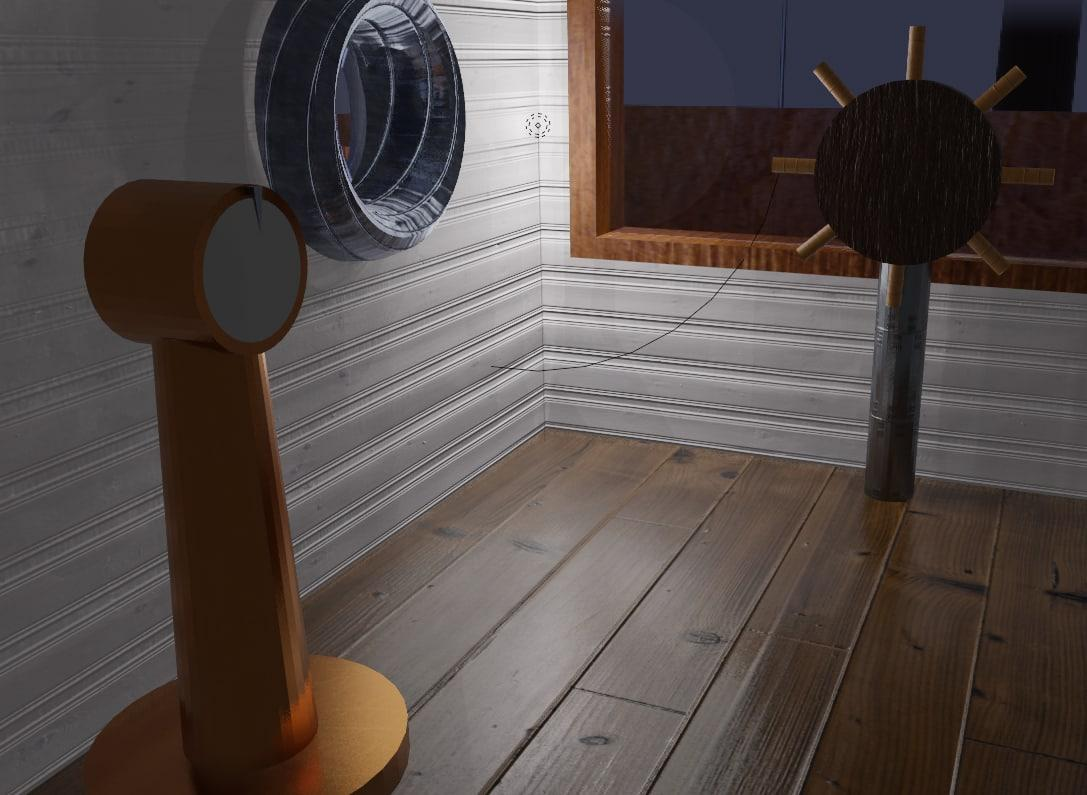
\includegraphics[scale=0.5]{imagens/timaotelegrafo.jpg}
    \caption{Timão e telégrafo renderizados.}
    \label{fig:tim_te}
\end{figure}

\begin{figure}[!h]
    \centering
    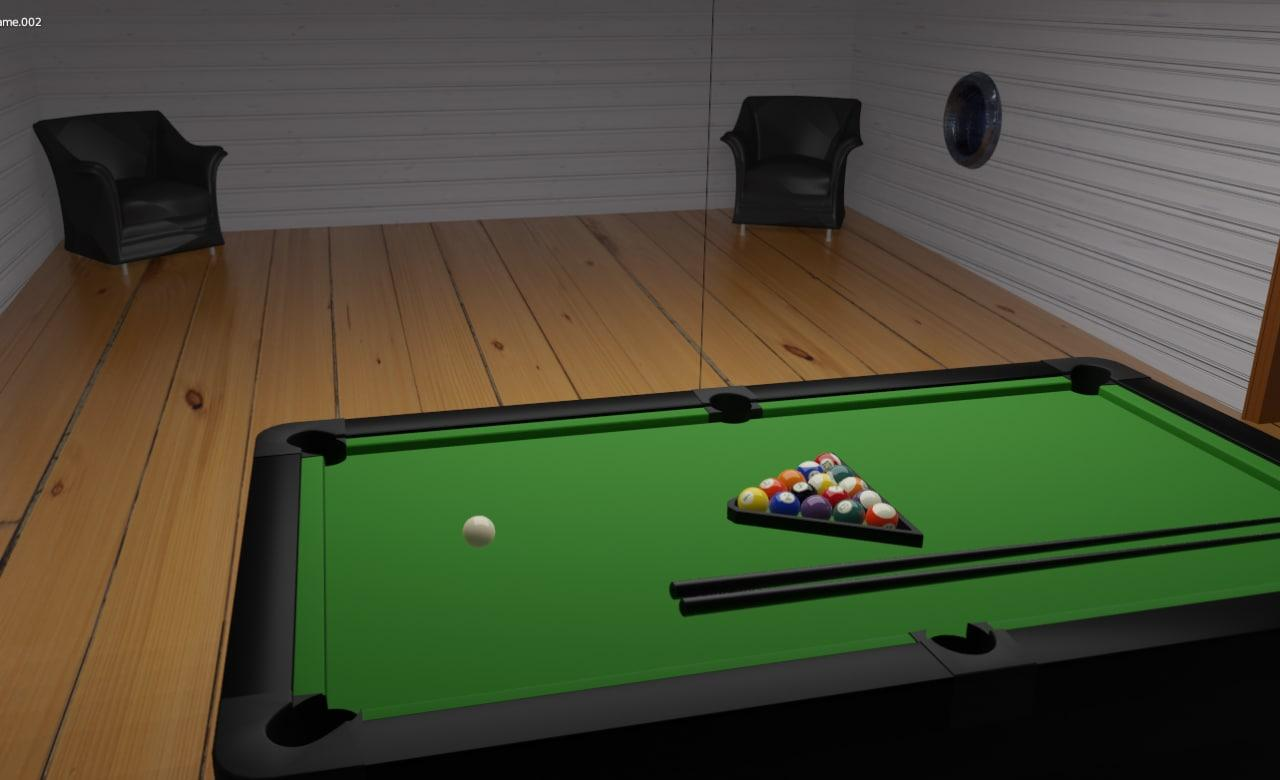
\includegraphics[scale=0.4]{imagens/sala1.jpg}
    \caption{Primeira sala do primeiro andar renderizada.}
    \label{fig:sala1}
\end{figure}


\begin{figure}[!h]
    \centering
    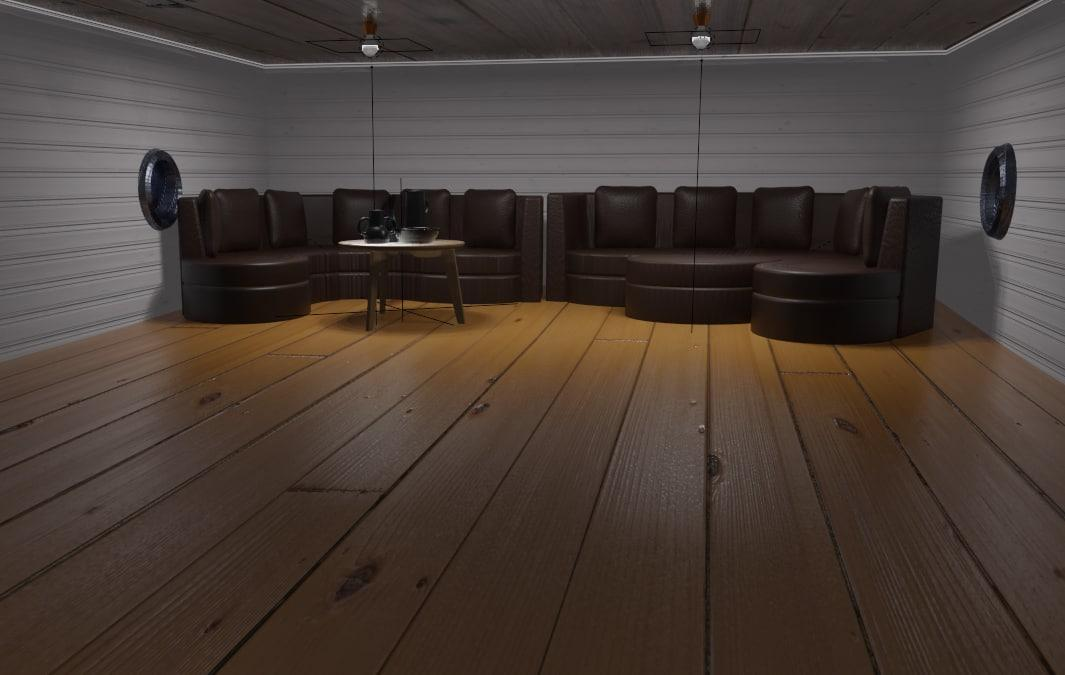
\includegraphics[scale=0.5]{imagens/sala2.jpg}
    \caption{Segunda sala do primeiro andar renderizada.}
    \label{fig:sala2}
\end{figure}


\begin{figure}[!h]
    \centering
    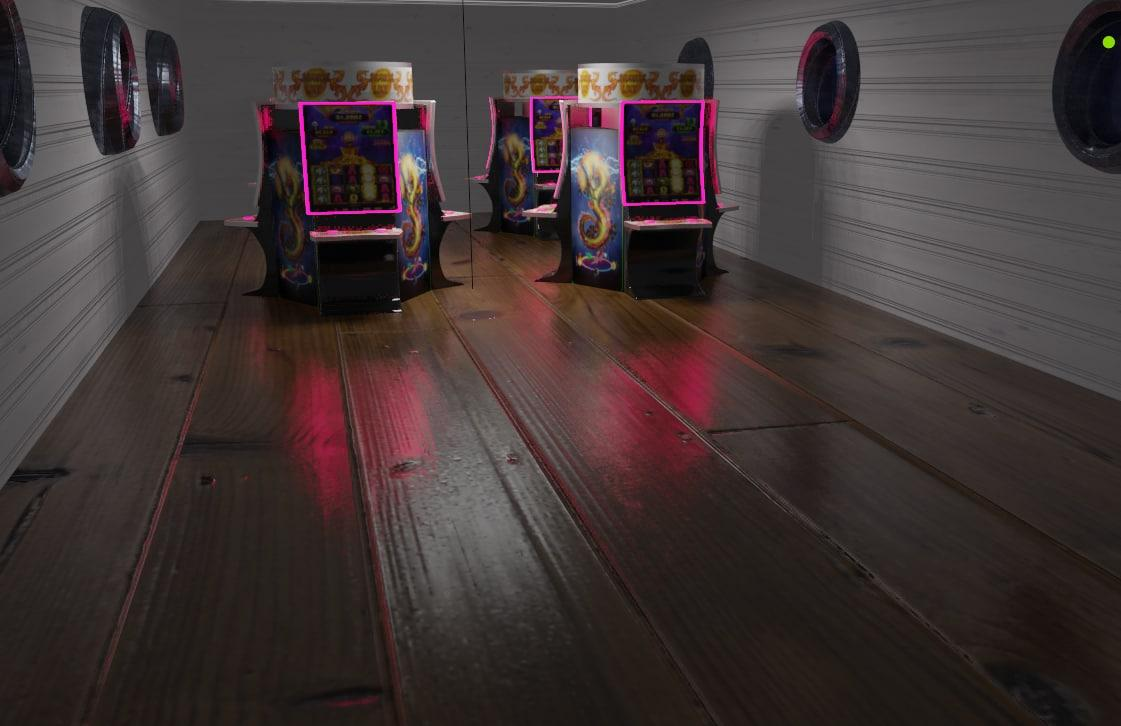
\includegraphics[scale=0.5]{imagens/sala.jpg}
    \caption{Sala do segundo andar renderizada.}
    \label{fig:niquel}
\end{figure}

As imagens \ref{fig:p1}, \ref{fig:p2}, \ref{fig:p3}, \ref{fig:p4}, \ref{fig:p5}, \ref{fig:p6}, \ref{fig:p7} e \ref{fig:p8} retratam um pouco do processo de desenvolvimento do projeto pelo grupo, desde as primeiras estruturas criadas até o início da aplicação das texturas.

\begin{figure}[!h]
    \centering
    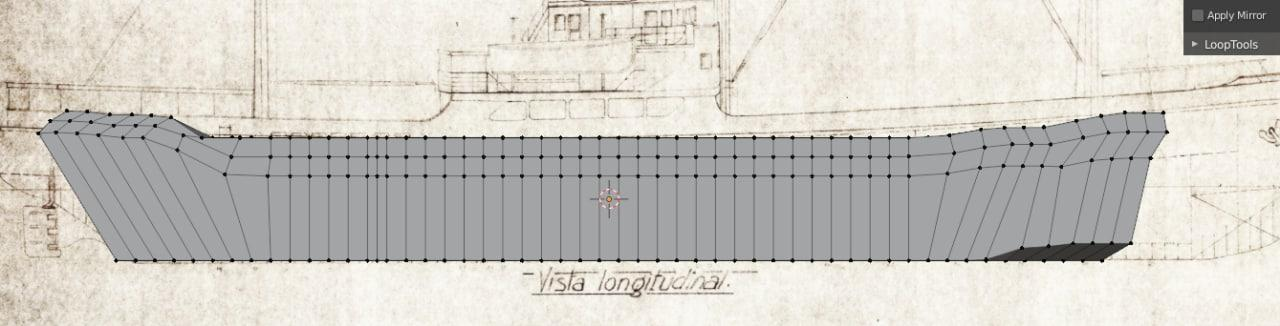
\includegraphics[scale=0.4]{imagens/p1.jpg}
    \caption{Processo de desenvolvimento.}
    \label{fig:p1}
\end{figure}

\begin{figure}[!h]
    \centering
    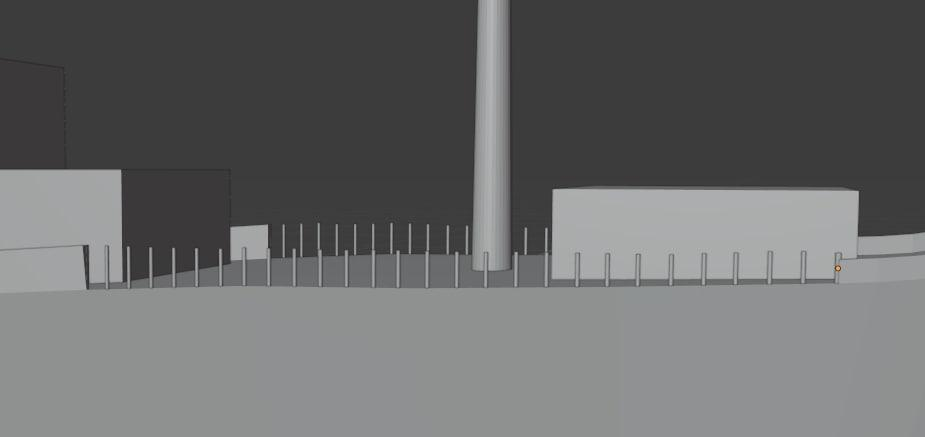
\includegraphics[scale=0.5]{imagens/p2.jpg}
    \caption{Processo de desenvolvimento.}
    \label{fig:p2}
\end{figure}

\begin{figure}[!h]
    \centering
    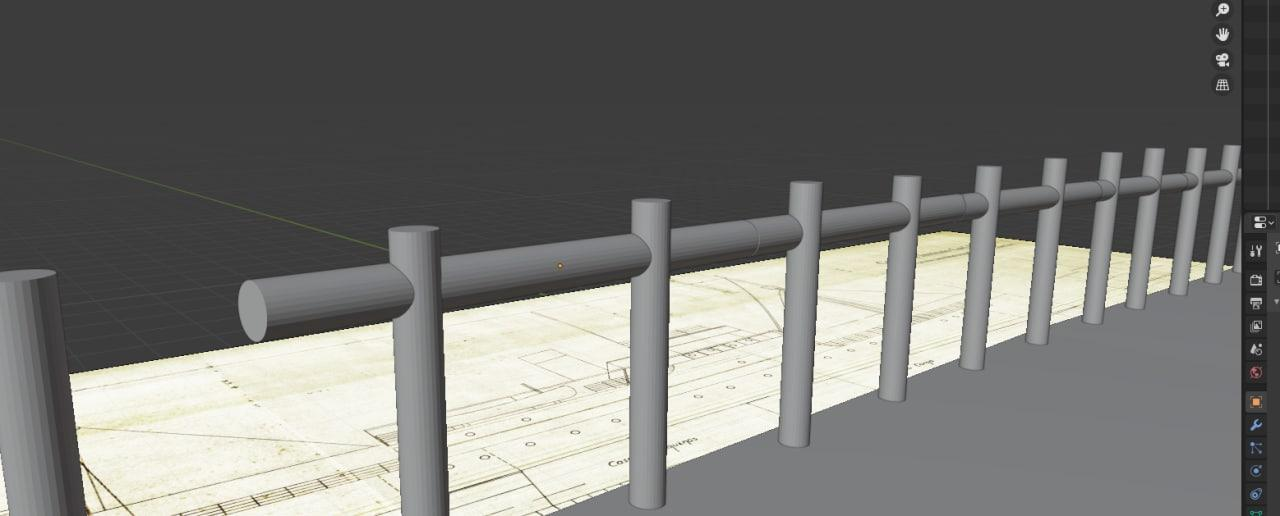
\includegraphics[scale=0.4]{imagens/p3.jpg}
    \caption{Processo de desenvolvimento.}
    \label{fig:p3}
\end{figure}

\begin{figure}[!h]
    \centering
    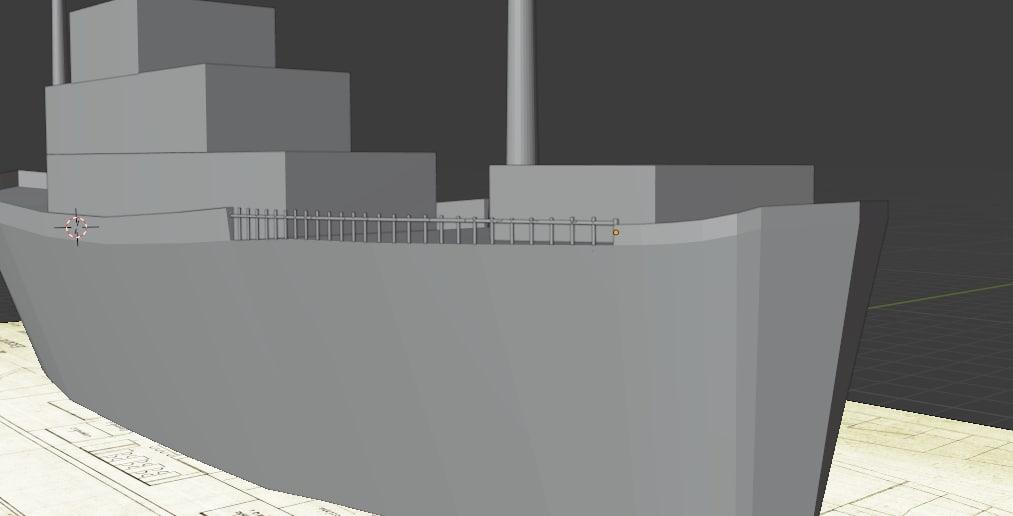
\includegraphics[scale=0.5]{imagens/p4.jpg}
    \caption{Processo de desenvolvimento.}
    \label{fig:p4}
\end{figure}

\begin{figure}[!h]
    \centering
    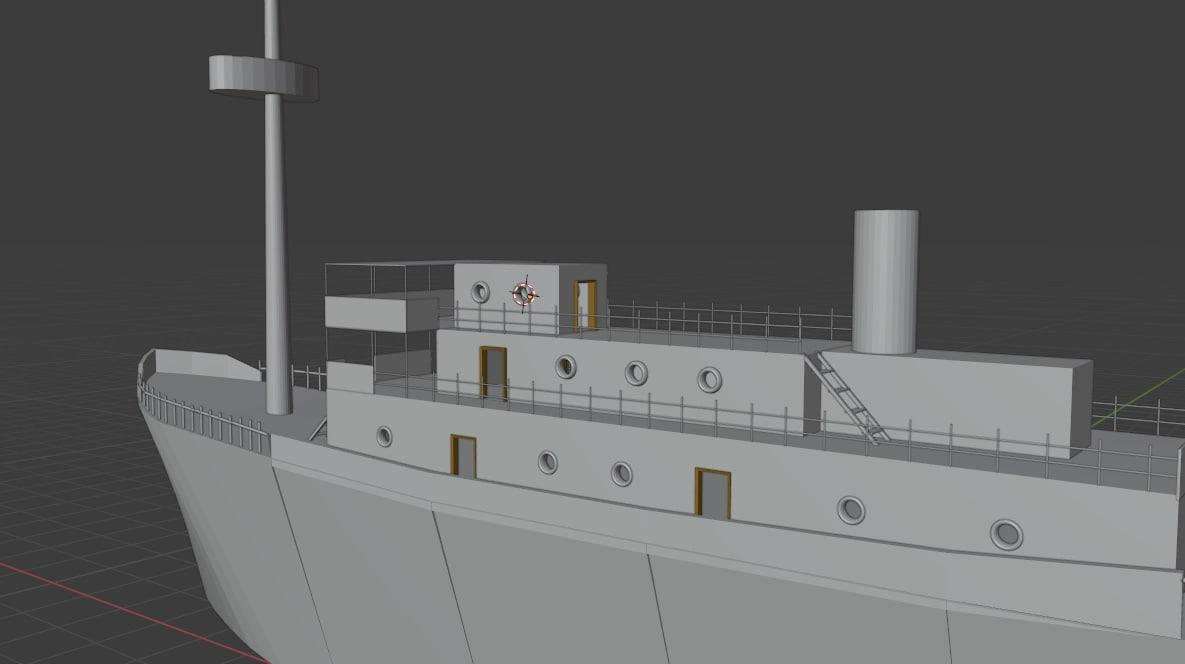
\includegraphics[scale=0.5]{imagens/p5.jpg}
    \caption{Processo de desenvolvimento.}
    \label{fig:p5}
\end{figure}

\begin{figure}[!h]
    \centering
    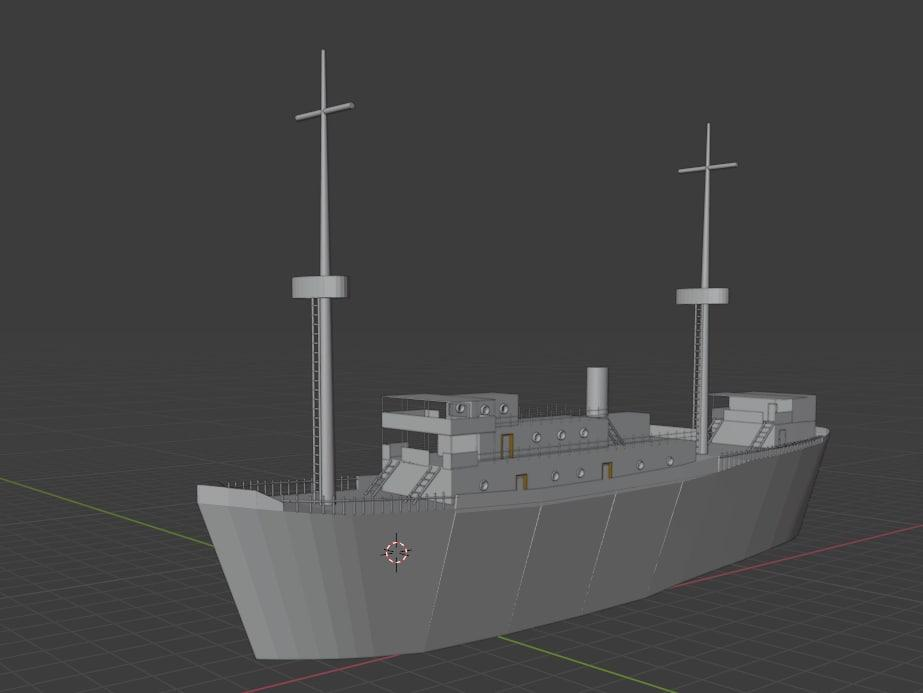
\includegraphics[scale=0.5]{imagens/p6.jpg}
    \caption{Processo de desenvolvimento.}
    \label{fig:p6}
\end{figure}

\begin{figure}[!h]
    \centering
    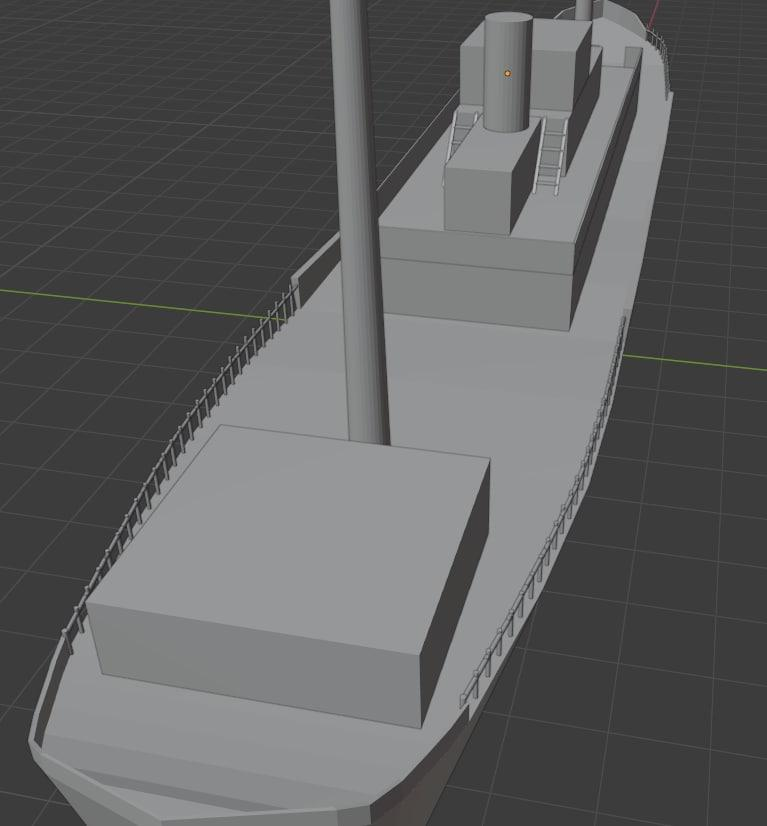
\includegraphics[scale=0.5]{imagens/p7.jpg}
    \caption{Processo de desenvolvimento.}
    \label{fig:p7}
\end{figure}

\begin{figure}[!h]
    \centering
    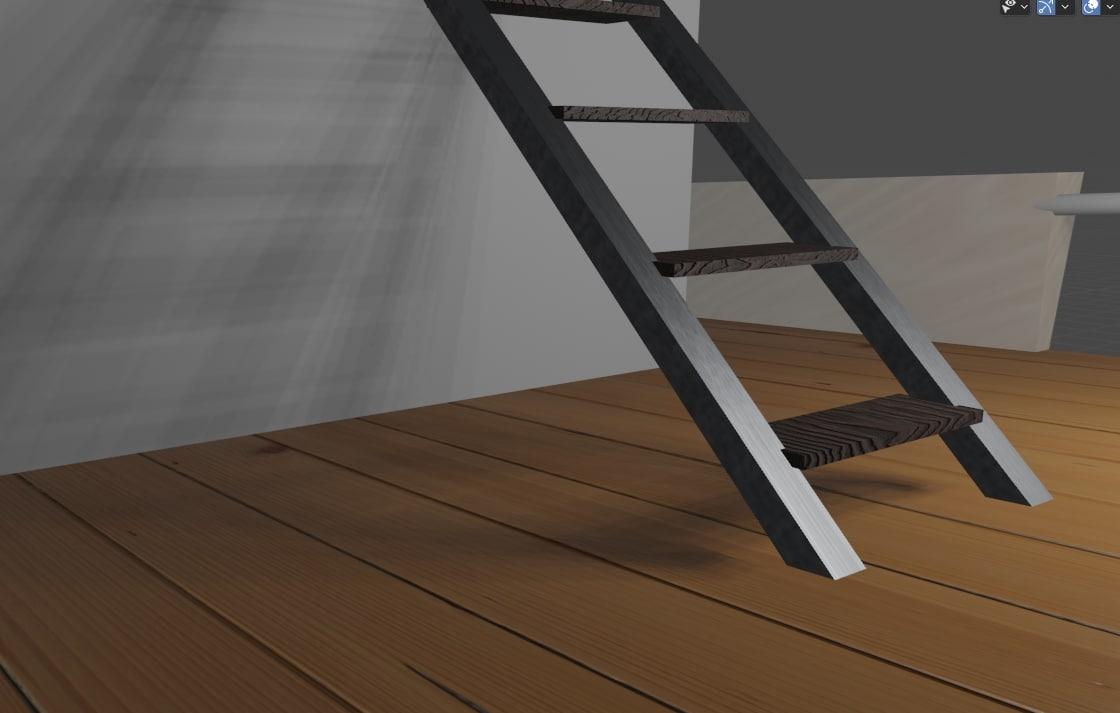
\includegraphics[scale=0.5]{imagens/p8.jpg}
    \caption{Processo de desenvolvimento.}
    \label{fig:p8}
\end{figure}

A figura \ref{fig:pf} apresenta o produto final do projeto, com as texturas aplicadas e o navio renderizado. Além dos arquivos do projeto, um vídeo será encaminhado junto a este relatório, realizando a visita virtual. Os vídeos renderizados para a visita foram feitos com a \textit{render engine} Eevee, enquanto as imagens renderizadas em alta qualidade foram feitas com a cycles utilizando 2000 amostras.  

\begin{figure}[!h]
    \centering
    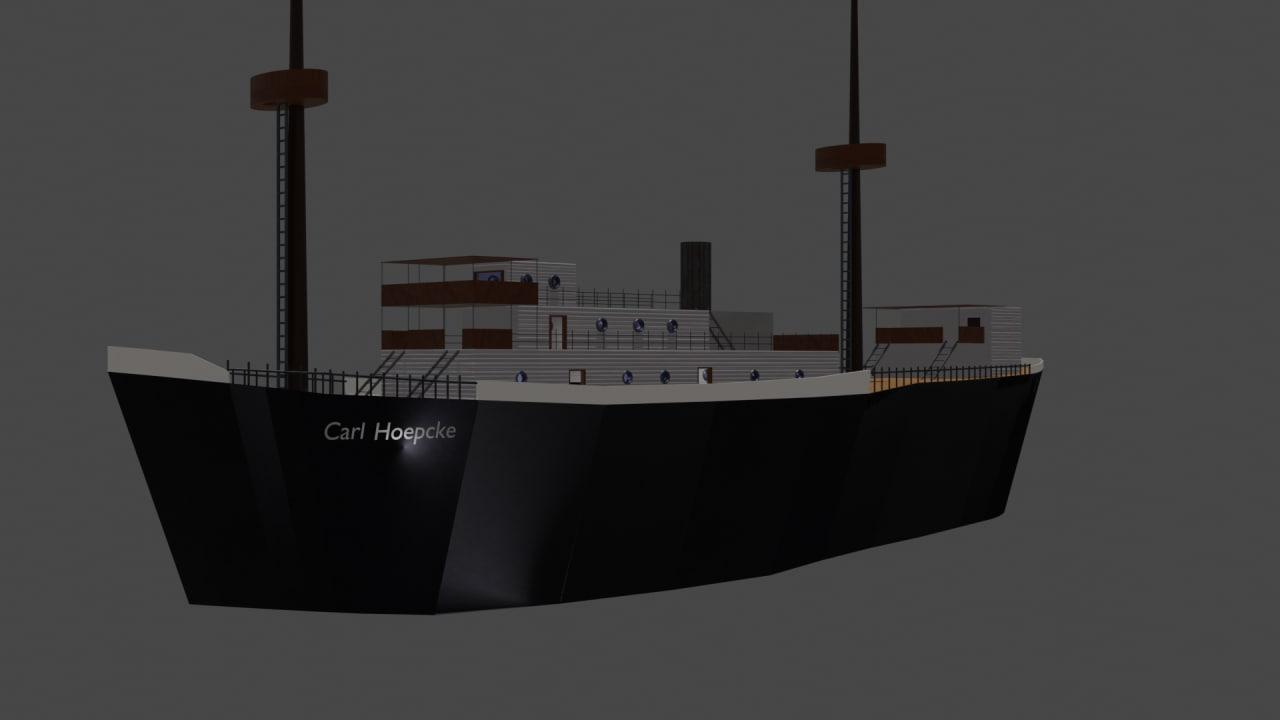
\includegraphics[scale=0.3]{imagens/render1.jpg}
    \caption{Produto final.}
    \label{fig:pf}
\end{figure}


% \bibliography{referencias}


\end{document}
